\documentclass[aspectratio=169,11pt]{beamer}

\usetheme{Madrid}
\usecolortheme{default}
\setbeamertemplate{navigation symbols}{}
\setbeamertemplate{footline}[frame number]

\usepackage{amsmath,amssymb}
\usepackage{graphicx}
\usepackage{tikz}
\usetikzlibrary{positioning,calc}
\usetikzlibrary{arrows.meta,decorations.pathmorphing}

\definecolor{RamRed}{RGB}{190,40,45}
\definecolor{RamBlue}{RGB}{30,90,180}
\definecolor{SoftGray}{RGB}{245,245,245}
\definecolor{DarkGray}{RGB}{70,70,70}
\definecolor{MapGreen}{RGB}{48,150,95}
\definecolor{MapGold}{RGB}{235,180,45}

\setbeamercolor{title}{fg=DarkGray}
\setbeamercolor{frametitle}{fg=white,bg=RamBlue}
\setbeamercolor{structure}{fg=RamBlue}

\tikzset{
  v/.style={circle,draw=black,fill=white,inner sep=1.8pt},
  edge/.style={draw=RamBlue,line width=1.25pt},
  topic/.style={draw=black!30,fill=SoftGray,rounded corners=5pt,inner sep=7pt,
    text width=5.8cm,minimum height=1.65cm,align=left},
}


\usepackage{booktabs}
\tikzset{dot/.style={circle,fill=black,inner sep=2pt}, lab/.style={circle,draw=black,fill=white,inner sep=2pt,minimum size=6mm,font=\small},selected/.style={draw=RamRed,line width=2pt}}

\newcommand{\Def}[2]{\begin{block}{#1}#2\end{block}}
\newcommand{\Thm}[2]{\begin{block}{#1}#2\end{block}}
\renewcommand{\Proof}[1]{\begin{block}{Proof}\normalsize #1\end{block}}
\newcommand{\Question}[1]{\begin{block}{Question}#1\end{block}}
\renewcommand{\Example}[1]{\begin{block}{Example}#1\end{block}}
\newcommand{\fall}[2]{#1^{\underline{#2}}}
\newcommand{\rise}[2]{#1^{\overline{#2}}}
\newcommand{\stir}[2]{\left\{\begin{matrix}#1\\#2\end{matrix}\right\}}
\newcommand{\cyc}[2]{\left[\begin{matrix}#1\\#2\end{matrix}\right]}
\newcommand{\eul}[2]{\left\langle\begin{matrix}#1\\#2\end{matrix}\right\rangle}
\newcommand{\coef}[2]{[#1^{#2}]}
\newcommand{\gap}{\par\medskip}

\title{Permutation Groups and Burnside\textquotesingle s Lemma}
\author{Jeremy Quastel}\date{}\begin{document}
\begin{frame}[plain]\begin{center}{\Huge\bfseries Permutation Groups and Burnside\textquotesingle s Lemma}\par\vspace{.25cm}{\Large Section 2.7.1--2.7.2}\par\vspace{.15cm}{\large Harris--Hirst--Mossinghoff, \emph{Combinatorics and Graph Theory}}\par\vspace{.1cm}\resizebox{!}{2.7cm}{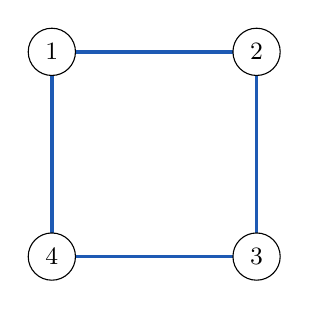
\begin{tikzpicture}[scale=1]
\coordinate (v1) at (-1.300,1.300);
\coordinate (v2) at (1.300,1.300);
\coordinate (v3) at (1.300,-1.300);
\coordinate (v4) at (-1.300,-1.300);
\draw[edge] (v1)--(v2);
\draw[edge] (v2)--(v3);
\draw[edge] (v3)--(v4);
\draw[edge] (v4)--(v1);
\node[lab] at (v1) {1};
\node[lab] at (v2) {2};
\node[lab] at (v3) {3};
\node[lab] at (v4) {4};
\end{tikzpicture}}\par\vspace{.25cm}Jeremy Quastel\end{center}\end{frame}
\begin{frame}[plain]\large \begin{center}{\Huge\bfseries Today\textquotesingle s lecture}\par\vspace{.5cm}\end{center}\begin{columns}[c,onlytextwidth]\begin{column}{.48\textwidth}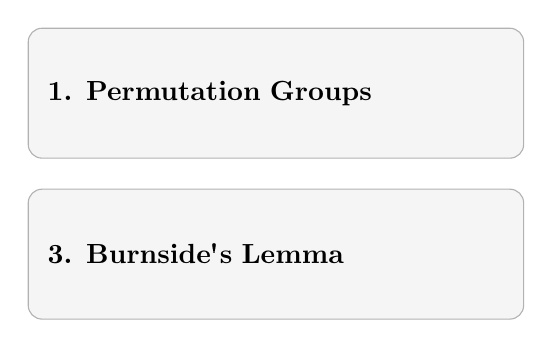
\begin{tikzpicture}\node[topic](a){\textbf{1. Permutation Groups}};\node[topic,below=.38cm of a]{\textbf{3. Burnside\textquotesingle s Lemma}};\end{tikzpicture}\end{column}\begin{column}{.48\textwidth}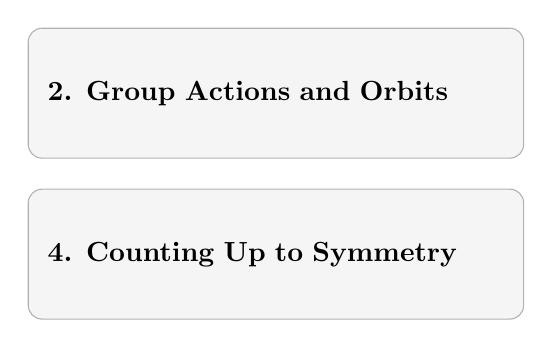
\begin{tikzpicture}\node[topic](a){\textbf{2. Group Actions and Orbits}};\node[topic,below=.38cm of a]{\textbf{4. Counting Up to Symmetry}};\end{tikzpicture}\end{column}\end{columns}\end{frame}
\begin{frame}{Section 2.7.1: Permutation groups}
\large
\Question{How many different colorings of a square are there when rotations or reflections may make two colorings equivalent?}
\begin{center}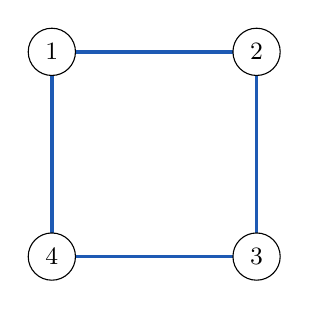
\begin{tikzpicture}[scale=1]
\coordinate (v1) at (-1.300,1.300);
\coordinate (v2) at (1.300,1.300);
\coordinate (v3) at (1.300,-1.300);
\coordinate (v4) at (-1.300,-1.300);
\draw[edge] (v1)--(v2);
\draw[edge] (v2)--(v3);
\draw[edge] (v3)--(v4);
\draw[edge] (v4)--(v1);
\node[lab] at (v1) {1};
\node[lab] at (v2) {2};
\node[lab] at (v3) {3};
\node[lab] at (v4) {4};
\end{tikzpicture}\end{center}
\end{frame}
\begin{frame}{Permutations as functions}
\large
\Def{Permutation}{A permutation of a finite set $X$ is a bijection from $X$ to itself. The permutations of $[n]$ form the symmetric group $S_n$.}
\gap A permutation can be written in two-row notation or as a product of disjoint cycles.
\end{frame}
\begin{frame}{Cycle notation}
\large
\Example{The permutation
\[\begin{pmatrix}1&2&3&4&5\\3&1&2&5&4\end{pmatrix}
\]
is $(1\ 3\ 2)(4\ 5)$.}
\gap A cycle $(a_1\ a_2\ \cdots\ a_k)$ sends $a_i$ to $a_{i+1}$ and $a_k$ to $a_1$. Fixed points may be written as one-cycles or omitted.
\end{frame}
\begin{frame}{Composing permutations}
\large
\Def{Convention}{In a product $\sigma\tau$, apply $\tau$ first and then $\sigma$.}
\Example{Let $\sigma=(1\ 2\ 3)$ and $\tau=(1\ 2)$. Then
\[\sigma\tau=(1\ 3),\qquad\tau\sigma=(2\ 3).\]}
\gap In general, permutation multiplication is not commutative.
\end{frame}
\begin{frame}{Groups}
\large
\Def{Group}{A set $G$ with a multiplication is a group if multiplication is associative, there is an identity element $e$, and each element has an inverse. The product of elements of $G$ must remain in $G$.}
\gap Permutations form groups under composition. The identity fixes every point, and the inverse reverses the bijection.
\end{frame}
\begin{frame}{Permutation groups}
\large
\Def{Permutation group}{A subgroup of $S_n$ is a collection of permutations containing the identity and closed under composition and inverses.}
\gap Geometric symmetries act by permuting vertices, edges, faces, or other positions.
\end{frame}
\begin{frame}{Rotations of a square}
\large
Let $r=(1\ 2\ 3\ 4)$. The rotation group is
\[C_4=\{e,r,r^2,r^3\},\qquad r^4=e.\]
\gap The rotations are by $0^\circ,90^\circ,180^\circ,270^\circ$ in the direction of the vertex labeling.
\end{frame}
\begin{frame}{All symmetries of a square}
\large
\Def{Dihedral group}{The group $D_4$ has eight elements: four rotations and four reflections. If $s$ is a reflection, then
\[D_4=\{e,r,r^2,r^3,s,rs,r^2s,r^3s\},\]
with $r^4=s^2=e$ and $srs=r^{-1}$.}
\gap The allowed symmetry group is part of the counting problem.
\end{frame}
\begin{frame}{Group actions}
\large
\Def{Action}{An action of a group $G$ on a set $X$ assigns an element $g\cdot x\in X$ to every $g\in G,x\in X$, with
\[e\cdot x=x,\qquad (gh)\cdot x=g\cdot(h\cdot x).\]}
\gap For us, $X$ will often be a set of colorings and $G$ a geometric symmetry group.
\end{frame}
\begin{frame}{Acting on colorings}
\large
A coloring of a position set $V$ with $k$ colors is a function $f:V\to[k]$.
\gap A permutation $g$ of $V$ acts by moving colors with their positions:
\[(g\cdot f)(v)=f(g^{-1}v).\]
\gap This convention ensures $(gh)\cdot f=g\cdot(h\cdot f)$.
\end{frame}
\begin{frame}{Orbits}
\large
\Def{Orbit}{The orbit of $x\in X$ is
\[\operatorname{Orb}(x)=\{g\cdot x:g\in G\}.\]}
\gap Two objects are equivalent under the allowed symmetries exactly when they lie in the same orbit.
\gap Orbits partition $X$ into disjoint equivalence classes.
\end{frame}
\begin{frame}{Stabilizers}
\large
\Def{Stabilizer}{The stabilizer of $x$ is
\[G_x=\{g\in G:g\cdot x=x\}.\]}
\gap It is a subgroup of $G$. Its elements are the symmetries that preserve the particular object $x$.
\end{frame}
\begin{frame}{The orbit--stabilizer theorem}
\large
\Thm{Theorem}{For a finite group acting on a set,
\[|\operatorname{Orb}(x)|=\frac{|G|}{|G_x|}.\]}
\gap Objects with more symmetry have smaller orbits.
\end{frame}
\begin{frame}{Proof of orbit--stabilizer}
\large
\Proof{Map $G$ onto $\operatorname{Orb}(x)$ by $g\mapsto g\cdot x$.\gap If $g\cdot x=h\cdot x$, then $h^{-1}g\in G_x$, so the elements sending $x$ to $h\cdot x$ are precisely $hG_x$. Each fiber therefore has $|G_x|$ elements.\gap The $|G|$ elements of the group split into $|\operatorname{Orb}(x)|$ equal fibers.}
\end{frame}
\begin{frame}{Why dividing by the group size fails}
\large
\Example{Color the square's vertices red or blue and allow rotations. An all-red coloring has orbit size $1$. A coloring with just one red vertex has orbit size $4$. An alternating coloring has orbit size $2$.}
\gap Since orbit sizes vary, dividing the $2^4$ labeled colorings by $4$ does not count the orbits.
\end{frame}
\begin{frame}{Section 2.7.2: Burnside's lemma}
\large
\Def{Fixed objects}{For $g\in G$, write
\[\operatorname{Fix}(g)=\{x\in X:g\cdot x=x\}.\]}
\Thm{Burnside's lemma}{The number of orbits of a finite group $G$ on a finite set $X$ is
\[\frac1{|G|}\sum_{g\in G}|\operatorname{Fix}(g)|.\]}
\end{frame}
\begin{frame}{Proof: count fixed pairs}
\large
\Proof{Count pairs $(g,x)\in G\times X$ for which $g\cdot x=x$. Counting first by $g$ gives
\[\sum_{g\in G}|\operatorname{Fix}(g)|.\]
Counting first by $x$ gives
\[\sum_{x\in X}|G_x|.\]}
\end{frame}
\begin{frame}{Proof: group the objects by orbit}
\large
\Proof{Within an orbit $O$, orbit--stabilizer gives $|G_x|=|G|/|O|$ for every $x\in O$. Therefore
\[\sum_{x\in O}|G_x|=|O|\frac{|G|}{|O|}=|G|.\]
Each orbit contributes exactly $|G|$ fixed pairs. Divide the total by $|G|$ to obtain the number of orbits.}
\end{frame}
\begin{frame}{Fixed colorings and cycles}
\large
\Thm{Key observation}{If a permutation of the positions has $c$ cycles, including fixed points, then it fixes exactly $k^c$ colorings with $k$ available colors.}
\Proof{A fixed coloring must be constant on each cycle. Choose its color independently for each of the $c$ cycles.}
\end{frame}
\begin{frame}{Square colorings up to rotation}
\large
\begin{center}\renewcommand{\arraystretch}{1.5}
\begin{tabular}{lcc}
Rotation & Cycles on vertices & Fixed colorings\\\hline
Identity &4&$k^4$\\
$90^\circ,270^\circ$ &1 each&$k$ each\\
$180^\circ$ &2&$k^2$
\end{tabular}\end{center}
\[\text{Number of orbits}=\frac{k^4+k^2+2k}{4}.\]
\end{frame}
\begin{frame}{Two and three colors}
\large
With two available colors, rotation classes number
\[\frac{2^4+2^2+2\cdot2}{4}=6.\]
With three available colors, they number
\[\frac{3^4+3^2+2\cdot3}{4}=24.\]
\gap The colors are labeled; a symmetry moves positions, not color names.
\end{frame}
\begin{frame}{Reflections of the square}
\large
\begin{center}\renewcommand{\arraystretch}{1.5}
\begin{tabular}{lcc}
Reflection axis & Number & Cycles on vertices\\\hline
Through opposite vertices &2&3\\
Through opposite edge midpoints &2&2
\end{tabular}\end{center}
\gap The first type fixes two vertices and swaps the other two. The second type swaps two pairs.
\end{frame}
\begin{frame}{Square colorings up to all symmetries}
\large
\Thm{Formula}{Under $D_4$, the number of vertex-coloring orbits is
\[\frac{k^4+2k^3+3k^2+2k}{8}.\]}
\gap For $k=3$, this is $21$. Allowing reflections merges some of the $24$ rotation classes.
\end{frame}
\begin{frame}{A prescribed number of red vertices}
\large
\Question{How many square colorings with exactly two red and two blue vertices are there, up to all symmetries?}
\gap We must count fixed colorings satisfying the color inventory. The unrestricted count $2^c$ is no longer appropriate.
\end{frame}
\begin{frame}{Exactly two red vertices: fixed counts}
\large
\normalsize
\begin{center}\renewcommand{\arraystretch}{1.5}
\begin{tabular}{lcc}
Symmetry & Number & Fixed colorings each\\\hline
Identity&1&6\\
Quarter-turn&2&0\\
Half-turn&1&2\\
Vertex-axis reflection&2&2\\
Edge-axis reflection&2&2
\end{tabular}\end{center}
\gap Burnside gives $(6+2+4+4)/8=2$ orbits: red vertices adjacent or opposite.
\end{frame}
\begin{frame}{Necklaces with $n$ positions}
\large
\Def{Rotation equivalence}{A necklace here is a coloring of $n$ cyclic positions, with rotations identified but reflections kept distinct.}
\gap Rotation by $j$ positions has $\gcd(n,j)$ cycles, taking $\gcd(n,0)=n$.
\[\text{Number of necklaces}=\frac1n\sum_{j=0}^{n-1}k^{\gcd(n,j)}.\]
\end{frame}
\begin{frame}{Why the gcd counts cycles}
\large
\Proof{Under rotation by $j$, a position returns after the least positive number $\ell$ such that $\ell j\equiv0\pmod n$. This is $\ell=n/\gcd(n,j)$.\gap All cycles have this length, so their number is $n/\ell=\gcd(n,j)$.}
\end{frame}
\begin{frame}{Prime-length necklaces}
\large
\Thm{Formula}{For prime $p$, the number of $k$-color necklaces is
\[\frac{k^p+(p-1)k}{p}.\]}
\gap The identity has $p$ cycles, and every nonidentity rotation has one cycle.
\gap Since the count is integral, $p$ divides $k^p-k$.
\end{frame}
\begin{frame}{Coloring the faces of a cube}
\large
\Question{How many face colorings of a cube are there up to rotation, using $k$ available colors?}
\begin{center}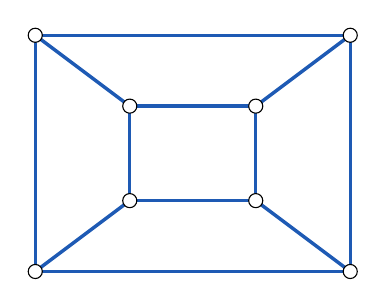
\begin{tikzpicture}[scale=1]
\coordinate (v1) at (-2.000,-1.500);
\coordinate (v2) at (2.000,-1.500);
\coordinate (v3) at (2.000,1.500);
\coordinate (v4) at (-2.000,1.500);
\coordinate (v5) at (-0.800,-0.600);
\coordinate (v6) at (0.800,-0.600);
\coordinate (v7) at (0.800,0.600);
\coordinate (v8) at (-0.800,0.600);
\draw[edge] (v1)--(v2);
\draw[edge] (v2)--(v3);
\draw[edge] (v3)--(v4);
\draw[edge] (v4)--(v1);
\draw[edge] (v5)--(v6);
\draw[edge] (v6)--(v7);
\draw[edge] (v7)--(v8);
\draw[edge] (v8)--(v5);
\draw[edge] (v1)--(v5);
\draw[edge] (v2)--(v6);
\draw[edge] (v3)--(v7);
\draw[edge] (v4)--(v8);
\node[v] at (v1) {};
\node[v] at (v2) {};
\node[v] at (v3) {};
\node[v] at (v4) {};
\node[v] at (v5) {};
\node[v] at (v6) {};
\node[v] at (v7) {};
\node[v] at (v8) {};
\end{tikzpicture}\end{center}
\end{frame}
\begin{frame}{The cube rotation group}
\large
\normalsize
There are $24$ rotations: choose the image of one face in $6$ ways, then the orientation around its normal in $4$ ways.
\begin{center}\renewcommand{\arraystretch}{1.3}
\begin{tabular}{lcc}
Rotation type & Number & Face-cycle lengths\\\hline
Identity&1&$1,1,1,1,1,1$\\
Face axis, quarter-turn&6&$1,1,4$\\
Face axis, half-turn&3&$1,1,2,2$\\
Vertex axis, third-turn&8&$3,3$\\
Edge axis, half-turn&6&$2,2,2$
\end{tabular}\end{center}
\end{frame}
\begin{frame}{Applying Burnside to cube faces}
\large
\Thm{Formula}{The number of face-coloring orbits under rotations is
\[\frac{k^6+3k^4+12k^3+8k^2}{24}.\]}
\gap With two colors, the answer is
\[\frac{64+48+96+32}{24}=10.\]
\end{frame}
\begin{frame}{A checklist for orbit counting}
\large
\begin{enumerate}
\item Specify the objects and the allowed symmetry group.
\item Classify the group elements by their action on positions.
\item Count the objects fixed by each element.
\item Average the fixed counts using Burnside's lemma.
\end{enumerate}
\gap If color counts or other restrictions are imposed, include them in step 3.
\end{frame}
\begin{frame}{Practice}
\large
\Question{How many colorings of the vertices of an equilateral triangle with $k$ colors are there up to rotation? What changes if reflections are also allowed?}
\end{frame}
\begin{frame}{Practice: solution}
\large
\normalsize
For rotations, the identity fixes $k^3$ colorings and the two nonidentity rotations each fix $k$:
\[\frac{k^3+2k}{3}.\]
For all six symmetries, the three reflections each have two vertex cycles and fix $k^2$ colorings:
\[\frac{k^3+3k^2+2k}{6}=\binom{k+2}{3}.\]
\end{frame}
\begin{frame}{Summary}
\large
\begin{itemize}
\item Group actions describe equivalence under symmetry.
\item Orbit--stabilizer relates an object's symmetries to its orbit size.
\item Burnside's lemma counts orbits by averaging fixed objects.
\item For unrestricted colorings, a permutation with $c$ position cycles fixes $k^c$ colorings.
\end{itemize}
\end{frame}
\begin{frame}{Next time: Partitions and Special Numbers}\begin{center}{\Huge Partitions and Special Numbers}\end{center}\end{frame}
\end{document}